% 3 · Data and methods
\section{Data and methods}

\begin{frame}{Datasets}{}
  {\scriptsize\renewcommand{\arraystretch}{1.0}
  \begin{tabularx}{\textwidth}{@{}>{\bfseries}l >{\raggedright\arraybackslash}X@{}}
    \toprule
    Theme & Sources \\
    \midrule
    Sites and capacity & Epoch AI data centres (MW, timelines; 96 sites), geocoded with OpenStreetMap \\
    Electricity and efficiency & IEA (2025) global and regional; LBNL US 2014–2023; Masanet global 2010–2018; Uptime PUE survey 2007–2025 \\
    Carbon & Ember grid carbon intensity by country (2024) \\
    Water & WRI Aqueduct 4.0 (baseline, 2030, 2050); WUE, PUE and grid water-intensity ranges (de Vries-Gao 2026); city records and news reports (case studies) \\
    Population & GHSL population grid (people near sites); UN World Population Prospects 2024 (capacity per person) \\
    Materials and waste & USGS Mineral Commodity Summaries 2026; Global E-waste Monitor 2024 \\
    Planetary boundaries & Stockholm Resilience Centre; Planetary Health Check 2025; Earth3 thresholds (Collste et al.\ 2018); Great Acceleration framing (Steffen et al.\ 2015) \\
    Society & Data Center Watch Q1 2026 (US); EJAtlas grievance categories; our two case studies \\
    \bottomrule
  \end{tabularx}}
  \par\smallskip
  {\scriptsize\textbf{Changes from the plan:} Epoch AI sites only (no all-data-centre layer or footprint model); 2 case
  studies, not 3–4 clusters; location quotients and country Gini in the report; per-internet-user Gini and a dispute
  catalogue not done; Great Acceleration shown with world energy only.\par}
  \note{%
    \NoteKey{Every number comes from a named public dataset or from our own scripts.}
    \NoteSlide{Sources by theme. The main ones: Epoch AI (96 AI data centres with power in MW, today and planned); IEA, LBNL
    and Masanet (electricity); Uptime Institute (PUE); Ember (grid carbon); WRI Aqueduct (water stress); GHSL (a 1 km
    population grid); USGS (minerals); the Global E-waste Monitor; Data Center Watch (opposition).}
    \NoteWhy{Epoch tracks only large AI sites, not all data centres, so each slide says which group a number refers to.}
    \NoteSay{30}{These are our datasets. The backbone is Epoch AI's database of 96 AI data centres with their power today
    and planned to 2030. Around it we use standard sources: the IEA and Lawrence Berkeley Lab for electricity, WRI's
    Aqueduct for water stress, the EU's population grid, and the US Geological Survey for minerals.}
    \begin{NoteAsk}
      \item \emph{Why only Epoch's sites?} It is the only open dataset with power and build timelines for each AI site.
    \end{NoteAsk}
  }
\end{frame}

\begin{frame}{Methods 1–2: where the capacity sits, and how unevenly}
  \begin{columns}[T,onlytextwidth]
    \column{.48\textwidth}
    \textbf{1\enspace Spatial overlay}
    \begin{itemize}\small
      \item 96 Epoch AI sites with reported MW (today and planned); geocode addresses (OpenStreetMap)
      \item Join to Aqueduct basins; count people within 25 and 50 km (GHSL grid)
      \item Output: \textbf{size-weighted} share of capacity in high water stress, now and in 2030/2050
    \end{itemize}
    \column{.48\textwidth}
    \textbf{2\enspace Inequality}
    \begin{itemize}\small
      \item Location quotient of capacity $C$ against population $P$ (in the report):
    \end{itemize}
    \[ LQ_i = \frac{C_i / C}{P_i / P} \]
    \begin{itemize}\small
      \item Lorenz curve and Gini coefficient of capacity per person (seven country groups)
    \end{itemize}
  \end{columns}
  \note{%
    \NoteKey{Put each site on a map, read its basin's water stress and count the people nearby; then measure how unevenly
    capacity is spread.}
    \NoteSlide{Method 1, spatial overlay: find each site's coordinates, look up its river basin in Aqueduct, count people
    within 25 and 50 km. The key output is the share weighted by MW, not just a count of sites. Method 2, inequality: the
    location quotient (a country's share of capacity $\div$ its share of population; above 1 = more than its share), and
    the Lorenz curve and Gini (0 = perfectly even, 1 = everything in one place).}
    \NoteSay{35}{Method one is a map overlay: each data centre goes onto the water-stress map, and we weight by size, so a
    2-gigawatt campus counts more than a small site. We also count the people living nearby. Method two measures
    inequality, comparing each country's share of capacity with its share of the world's people.}
    \begin{NoteAsk}
      \item \emph{Where are the location quotients?} The country table with them comes in the final report; slide 5 shows
        capacity per person, the same idea.
    \end{NoteAsk}
  }
\end{frame}

\begin{frame}{Methods 3–4: how much water, and how fast it grows}
  \begin{columns}[T,onlytextwidth]
    \column{.48\textwidth}
    \textbf{3\enspace Water-use range}
    \[ W_{\text{direct}} = E_{\text{IT}} \times \text{WUE} \]
    \[ W_{\text{indirect}} = E_{\text{IT}} \times \text{PUE} \times WI_{\text{grid}} \]
    {\small Low and high bounds from published WUE, PUE and generation water-intensity ranges.\par}
    \column{.48\textwidth}
    \textbf{4\enspace Standardised growth}
    \[ \ln y_t = a + bt \]
    \[ r = e^{b}-1, \qquad T_2 = \frac{\ln 2}{b} \]
    {\small 95\% intervals where annual data exist; observed and projected years kept separate.
    A two-segment fit tests where the breakpoints fall in the long series (world energy, AI compute).\par}
  \end{columns}
  \note{%
    \NoteKey{We estimate water from electricity, and measure growth as percent per year and doubling time.}
    \NoteSlide{Method 3: direct water = computer energy $\times$ WUE (litres evaporated on site per kWh); indirect water =
    the building's energy $\times$ the water evaporated per kWh at power plants. Low and high bounds come from published
    ranges. Method 4: fit a straight line to the logarithm of the data. Its slope gives the annual growth $r$ and the
    doubling time $T_2$, with 95\% intervals where yearly data exist; a two-segment fit finds where the trend breaks.}
    \NoteWhy{Rule of thumb: doubling time $\approx$ 70 $\div$ growth in \% (7\% a year $\to$ about 10 years).}
    \NoteSay{35}{Method three estimates water from electricity: on-site cooling water, plus the water evaporated at power
    plants. We give a low and a high value, because published values vary a lot. Method four turns every trend into a
    growth rate and a doubling time, so the three phases can be compared on one scale.}
  }
\end{frame}

\begin{frame}{Method 5: case studies and synthesis}
  \begin{columns}[T,onlytextwidth]
    \column{.44\textwidth}
    \textbf{Two contrasting cases}
    \begin{itemize}\small
      \item Google Mesa, Arizona: on our map, extremely high stress
      \item Google–AdaniConneX Visakhapatnam, India: planned 1 GW, not yet in the Epoch data
    \end{itemize}
    \smallskip
    {\small For each: water source and distance, local reaction, and our own estimate, from news
    reports and official documents.\par}
    \medskip
    {\small All results feed one matrix: \textbf{planetary boundary × scale of impact}.\par}
    \column{.52\textwidth}
    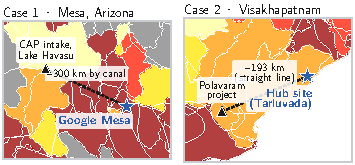
\includegraphics[width=\linewidth]{figs/case_locator.pdf}\par\smallskip
    {\scriptsize\color{muted} Star: data centre. Triangle: its water source. Background: Aqueduct
    baseline water stress (same colours as the results map).\par}
  \end{columns}
  \note{%
    \NoteKey{Two contrasting case studies, and one matrix that pulls everything together.}
    \NoteSlide{Google in Mesa, Arizona (a desert city, on our map, extremely high stress) and Google with AdaniConneX in
    Visakhapatnam, India (planned 1 GW, not yet in Epoch's data). On the map: star = data centre, triangle = its water
    source, colours = water stress. Mesa's river water travels about 300 km by canal; Vizag's promised source, Polavaram,
    is about 190 km away.}
    \NoteWhy{Totals hide places. Case studies show what the numbers mean on the ground.}
    \NoteSay{30}{Method five is two case studies, one in a US desert city and one in an Indian port city, built from news
    reports and official records. For each we look at where the water comes from, how far it travels, how people reacted,
    and our own estimate. Everything then feeds one matrix: planetary boundary by scale of impact.}
  }
\end{frame}
